\documentclass[12pt]{article}

\usepackage[utf8]{inputenc}
\usepackage{graphicx}
\usepackage{fancyhdr}
\usepackage{float}

\title{g55\_dealer - Pseudo-Random Card Dealer}
\author{Group 55\\Juliette Regimbal (260657238)\\Qingzhou Yang (260687570)}
\date{March 27, 2017}
\pagenumbering{gobble}
\pagenumbering{arabic}
\pagestyle{fancy}

\begin{document}
\maketitle
\setlength{\parindent}{0ex}
\lhead{Group 55}
\rhead{Juliette Regimbal (260657238)\\Qingzhou Yang (260687570)}
\section{Circuit Description}
The \textit{g55\_dealer} circuit is a finite state machine (FSM) that manages other components that together allow for a random card to be drawn from a standard 52 card deck held in a \textit{g55\_stack52} circuit. The circuit has four 1-bit inputs (\texttt{request\_deal}, \texttt{RAND\_LT\_NUM}, \texttt{reset}, and \texttt{clock}) and two 1-bit outputs (\texttt{stack\_enable} and \texttt{rand\_enable}). \texttt{request\_deal} is high when a random card is needed from the deck, \texttt{RAND\_LT\_NUM} is high if the pseudorandom number is less than the total number of cards in the deck, \texttt{reset} is the asynchronous reset, and \texttt{clock} is the clock signal for the entire circuit usually at 50 MHz. \texttt{stack\_enable} is a signal allowing operations to occur on the stack, namely the POP operation to fetch a card. \texttt{rand\_enable} is the signal to get a new pseudorandom number from \textit{g55\_randu}. \\

A pinout of the circuit is as follows:\\

\begin{figure}[H]
\centering
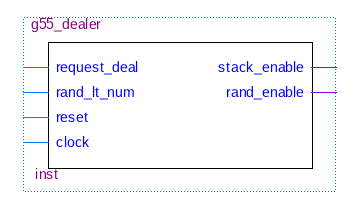
\includegraphics[scale=0.4]{graphics/dealer-pinout.png}
\caption{\textit{g55\_dealer} Pinout}
\end{figure}

\begin{table}[H]
\caption{\textit{g55\_dealer} Finite State Machine}
\centering
\begin{tabular}{c c | c c | c c}
\hline\hline
\multicolumn{2}{c |}{Inputs} & \multicolumn{2}{c |}{State} & \multicolumn{2}{c}{Outputs} \\
\hline
request\_deal & RAND\_LT\_NUM & State & Next State & stack\_enable & rand\_enable \\
\hline
0 & X & 00 & 01 & 0 & 0 \\
1 & X & 00 & 00 & 0 & 0 \\
0 & X & 01 & 01 & 0 & 0 \\
1 & X & 01 & 11 & 0 & 0 \\
X & 0 & 11 & 11 & 0 & 1 \\
X & 1 & 11 & 10 & 0 & 1 \\
X & X & 10 & 00 & 1 & 0 \\
\hline
\end{tabular}
\end{table}

\section{Testing}
The \textit{g55\_dealer} circuit was tested using a testbench and timing simulation. For the timing simulation, the circuit was stepped through the different states by varying the inputs as necessary. The delay in the circuit between a change in inputs and it being reflected in the simulation is clearly shown, and small enough to not cause any problems. The testbench was to test the \textit{g55\_dealer} with other components and start putting everything together for the Crazy Eights circuit. Since everything worked together with this basic form of the testbench only containing the stack, random number generator, a comparator circuit, and a seven segment decoder, the \textit{g55\_dealer} must be working as intended.

\begin{figure}[H]
\centering
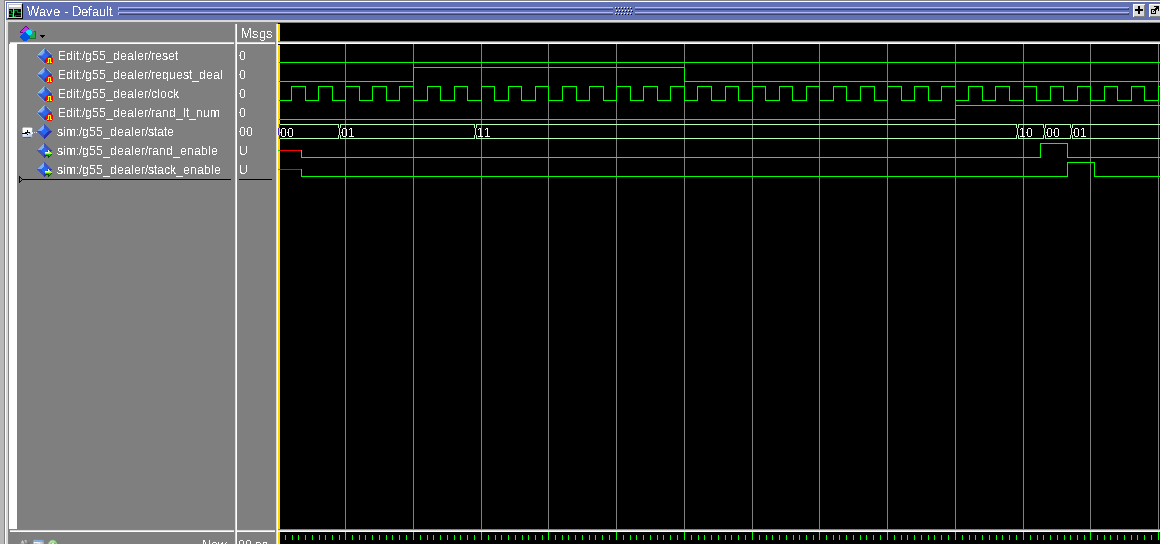
\includegraphics[scale=0.4]{graphics/dealer-sim.png}
\caption{\textit{g55\_dealer} Timing Simulation Results}
\end{figure}

\section{FPGA}
The \textit{g55\_dealer} circuit uses a total of 5 logic elements on the FPGA, 4 combinational functions, and 4 dedicated logic registors according to the Flow Summary generated after compilation. All of these represent a use of less than 1\% of FPGA resources. As there are six inputs and outputs, six of the pins must be used. The timing analysis shows positive slack for all connections, meaning signals pass through the system on all paths sufficiently fast for the circuit to work as desired. However the slack is small, so increasing the clock frequency by a significant amount would prevent the circuit from operating as intended.

\end{document}